\documentclass{beamer}

\usepackage[english]{babel}
\usepackage[utf8x]{inputenc}
\usepackage{comment}
\usepackage{array}
\usepackage{verbatim}
\usepackage{booktabs}
\usepackage{graphicx}
\usepackage{listings}
\usepackage{inconsolata}
\usepackage[sc]{mathpazo}
\usepackage[T1]{fontenc}
\usepackage{alltt}

\DefineNamedColor{named}{Black}           {cmyk}{0,0,0,1}
\DefineNamedColor{named}{Red}           {cmyk}{0,1,1,0}
\DefineNamedColor{named}{Green}         {cmyk}{1,0,1,0}
\DefineNamedColor{named}{LightGreen}          {cmyk}{0.2,0,0.2,0}
\DefineNamedColor{named}{LightRed}           {cmyk}{0,0.2,0.2,0}

\newcommand{\colorwrevert}[2]{\color{#1}#2\color{Black}}

\usepackage{caption3} % load caption package kernel first
\DeclareCaptionOption{parskip}[]{} % disable "parskip" caption option
\usepackage[small]{caption}

\mode<presentation>
{ 
	\usetheme{boxes} 
	\usecolortheme{seagull}
	\usefonttheme{serif}
}

\lstset {
	basicstyle=\footnotesize\ttfamily,
	basewidth=0.5em,
	language=bash,
	breaklines=true,
	breakatwhitespace=true
}

\usebackgroundtemplate{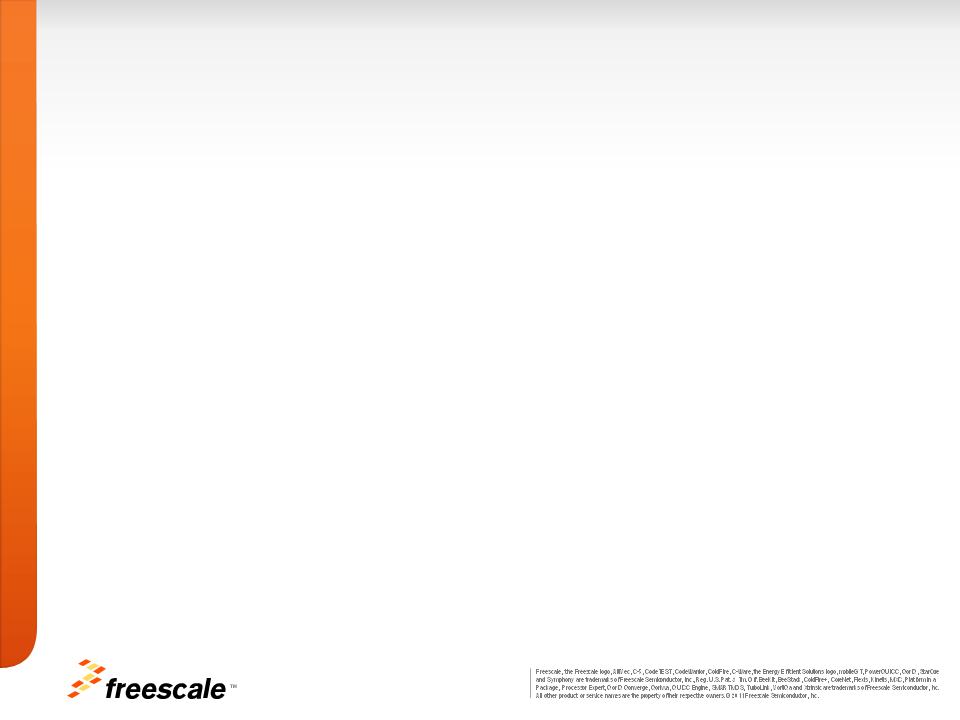
\includegraphics[width=\paperwidth]{img/back.png}}

\title{LinuX Containers}
% \subtitle{an overall approach}
\author{Bogdan Purc\u{a}rea\c{t}\u{a}}

\begin{document}

\setbeamertemplate{footline}[frame number]

\frame{\titlepage}

\frame{\tableofcontents}

\section{Concepts}

\subsection{Operating Systems}

\begin{frame}{IT trends}
	\begin{itemize}
		\item More resources
			\begin{itemize}
			\item Better hardware at lower costs
			\item Higher standards for software quality
			\end{itemize}
		\item More users
			\begin{itemize}
			\item Contact with technology at an earlier age
			\item Shared access to the same device
			\end{itemize}
		\item Data consolidation
			\begin{itemize}
			\item Data warehousing
			\item Service unification
			\item Differentiated access
			\end{itemize}
		\item Increased flexibility
			\begin{itemize}
			\item Versatile configuration
			\item Focus on usability
		\end{itemize}
	\end{itemize}
\end{frame}

\begin{frame}{OS Recap}
	\begin{columns}[T]
		\begin{column}{.5\textwidth}
			\begin{itemize}
			\item Resources
				\begin{itemize}
				\item CPU
				\item Memory
				\item Peripherals
				\end{itemize}
			\item Structures
				\begin{itemize}
				\item The scheduler
				\item The pager
				\item Filesystems
				\end{itemize}
			\item The kernel
				\begin{itemize}
				\item Handles hardware
				\item Exposes capabilities
				\item Manages resources
				\end{itemize}
			\end{itemize}
		\end{column}
		\begin{column}{.5\textwidth}
			\begin{figure}[ht]
				\vspace*{-0.7cm}
				\caption{The Memory Pager}
				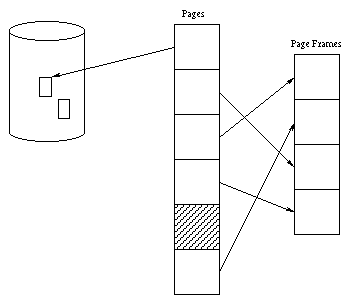
\includegraphics[height=0.3\textheight]{img/pager.png}
			\end{figure}
			\begin{figure}[ht]
				\vspace*{-0.7cm}
				\caption{The Scheduler}
				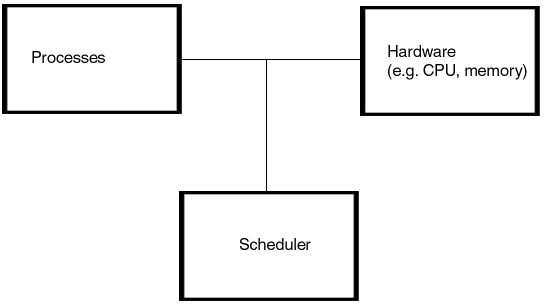
\includegraphics[height=0.3\textheight]{img/scheduler.png}
			\end{figure}
		\end{column}
	\end{columns}
\end{frame}

\subsection{Virtualization}

\begin{frame}{Virtualization}
	\begin{columns}[T]
		\begin{column}{.6\textwidth}
			\begin{itemize}
			\item Key aspects:
				\begin{itemize}
				\item Simulation (of HW / SW)
				\item Virtual machines
				\item Autonomous computing
				\item Utility computing
				\end{itemize}
			\item Advantages:
				\begin{itemize}
				\item Better resource usage
				\item Lower running costs
				\item Improved security
				\end{itemize}
			\item Concerns:
				\begin{itemize}
				\item Management
				\item Isolation
				\item Performance
				\item Applicability
				\end{itemize}
			\end{itemize}	
		\end{column}
		\begin{column}{.4\textwidth}
			\begin{figure}[hb]
				\centering
				
\includegraphics[width=\textwidth]{img/virt.png}
			\end{figure}
		\end{column}
	\end{columns}
\end{frame}

\begin{frame}{OS-level Virtualization}
	\begin{itemize}
	\item One host
	\item Multiple running OS instances
	\item Rootfs, system libs, binaries
	\end{itemize}
	
	OS instance = a process hierarchy
	
	OS level virtualization = \textbf{partitioning} the process tree
	
	Advantage: \textbf{close to 0\% performance overhead}
	
	Flaw: \textbf{shared kernel}
\end{frame}

\section{LinuX Containers}

\begin{frame}{LinuX Containers}
	\begin{columns}[T]
		\begin{column}{.6\textwidth}
			\begin{itemize}
			\item a.k.a. LXC:
				\begin{itemize}
				\item Mature technology implementation
				\item Mainline kernel support
				\item Application vs. System
				\item Active development
				\end{itemize}
			\item Components:
				\begin{itemize}
				\item \textit{Kernel features}
				\item \textit{Userspace tools}
				\item \textit{Configuration files}
				\item \textit{Template files}
				\end{itemize}
			\end{itemize}
		\end{column}
		\begin{column}{.4\textwidth}
			\begin{figure}[ht]
				\centering
				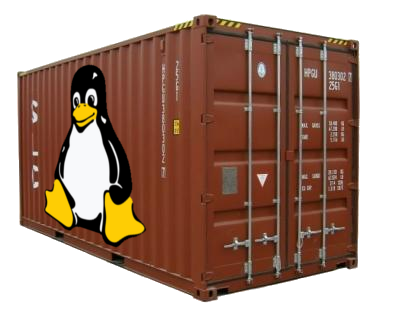
\includegraphics[width=\textwidth]{img/containers.png}
			\end{figure}
		\end{column}
	\end{columns}
\end{frame}

\begin{frame}{Kernel Support}
	\begin{columns}[C]
		\begin{column}{.6\textwidth}
			\begin{itemize}
			\setlength{\itemsep}{50pt}
			\item Namespaces:
				\begin{itemize}
				\item Abstract resources
				\item Processes see the resource as their own
				\item Isolation between namespaces
				\end{itemize}
			\item Control Groups
				\begin{itemize}
				\item Resource management among processes
				\item Hierarchical support
				\item Interaction with resource responsible structures:
					\begin{itemize}
					\item Scheduler
					\item Pager
					\end{itemize}
				\end{itemize}
			\end{itemize}	
		\end{column}
		\begin{column}{.4\textwidth}
			\begin{figure}[ht]
				\centering
				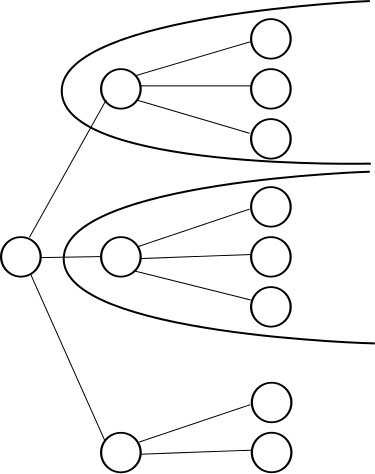
\includegraphics[scale=0.2]{img/namespaces.png}
			\end{figure}
			
			\begin{figure}[hb]
				\centering
				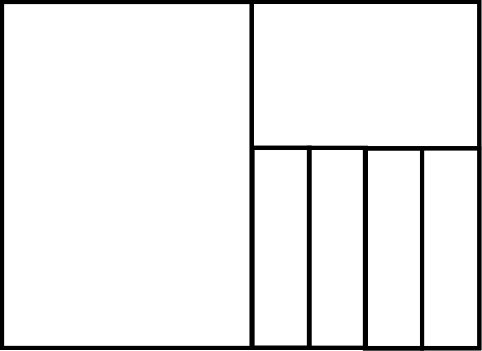
\includegraphics[scale=0.2]{img/cgroups.png}
			\end{figure}
		\end{column}
	\end{columns}
\end{frame}

\section{Usage}
\subsection{Schematics}

\begin{frame}[fragile]
\frametitle{Sample Process Hierarchy}
\begin{alltt}\footnotesize
init(1)-+-dnsmasq(2162)
        |-klogd(2175)
        |-lxc-start(2964)---init(2966)----+-init(2972)
        |                                 |-sh(2971)
        |                                 `-syslogd(2969)
        |
        |
        |-lxc-start(2974)---init(2976)----+-init(2982)
        |                                 |-sh(2981)
        |                                 `-syslogd(2979)
        |
        |
        |-netserver(2167)
        |-sh(2179)
        |-syslogd(2173)
        `-udevd(962)-+-udevd(1189)
                     `-udevd(1190)
\end{alltt}\normalsize
\end{frame}

\begin{frame}[fragile]
\frametitle{Process IDs}
\begin{alltt}\footnotesize
init(1)-+-dnsmasq(2162)
        |-klogd(2175)
        |-lxc-start(2964)---init(2966)\colorwrevert{Green}{(1)}-+-init(2972)\colorwrevert{Green}{(7)}
        |                                 |-sh(2971)\colorwrevert{Green}{(6)}
        |                                 `-syslogd(2969)\colorwrevert{Green}{(4)}
        |
        |
        |-lxc-start(2974)---init(2976)\colorwrevert{Red}{(1)}-+-init(2982)\colorwrevert{Red}{(7)}
        |                                 |-sh(2981)\colorwrevert{Red}{(6)}
        |                                 `-syslogd(2979)\colorwrevert{Red}{(4)}
        |
        |
        |-netserver(2167)
        |-sh(2179)
        |-syslogd(2173)
        `-udevd(962)-+-udevd(1189)
                     `-udevd(1190)
\end{alltt}\normalsize
\end{frame}

\begin{frame}[fragile]
\frametitle{Namespace Segregation}
\begin{alltt}\footnotesize
init(1)-+-dnsmasq(2162)
        |-klogd(2175)
        |-lxc-start(2964)---\colorbox{LightGreen}{init(2966)\colorwrevert{Green}{(1)}-+-init(2972)\colorwrevert{Green}{(7)}    }
        |                   \colorbox{LightGreen}{              |-sh(2971)\colorwrevert{Green}{(6)}      }
        |                   \colorbox{LightGreen}{              `-syslogd(2969)\colorwrevert{Green}{(4)} }
        |                   \colorwrevert{Green}{PID Namespace 1}
        |
        |-lxc-start(2974)---\colorbox{LightRed}{init(2976)\colorwrevert{Red}{(1)}-+-init(2982)\colorwrevert{Red}{(7)}    }
        |                   \colorbox{LightRed}{              |-sh(2981)\colorwrevert{Red}{(6)}      }
        |                   \colorbox{LightRed}{              `-syslogd(2979)\colorwrevert{Red}{(4)} }
        |                   \colorwrevert{Red}{PID Namespace 2}
        |
        |-netserver(2167)
        |-sh(2179)
        |-syslogd(2173)
        `-udevd(962)-+-udevd(1189)
                     `-udevd(1190)
\end{alltt}\normalsize
\end{frame}

\begin{frame}[fragile]
\frametitle{Filesystem Segregation}
\framesubtitle{"chroot on steroids"}
\begin{alltt}\footnotesize
init(1)-+-dnsmasq(2162)
        |-klogd(2175)       \colorwrevert{Green}{root: /var/lib/lxc/foo1/rootfs/}
        |-lxc-start(2964)---\colorbox{LightGreen}{init(2966)\colorwrevert{Green}{(1)}-+-init(2972)\colorwrevert{Green}{(7)}    }
        |                   \colorbox{LightGreen}{              |-sh(2971)\colorwrevert{Green}{(6)}      }
        |                   \colorbox{LightGreen}{              `-syslogd(2969)\colorwrevert{Green}{(4)} }
        |                   \colorwrevert{Green}{PID Namespace 1}
        |                   \colorwrevert{Red}{root: /var/lib/lxc/foo1/rootfs/}
        |-lxc-start(2974)---\colorbox{LightRed}{init(2976)\colorwrevert{Red}{(1)}-+-init(2982)\colorwrevert{Red}{(7)}    }
        |                   \colorbox{LightRed}{              |-sh(2981)\colorwrevert{Red}{(6)}      }
        |                   \colorbox{LightRed}{              `-syslogd(2979)\colorwrevert{Red}{(4)} }
        |                   \colorwrevert{Red}{PID Namespace 2}
        |
        |-netserver(2167)
        |-sh(2179)
        |-syslogd(2173)
        `-udevd(962)-+-udevd(1189)
                     `-udevd(1190)
\end{alltt}\normalsize
\end{frame}

\begin{frame}[fragile]
\frametitle{CPU Partitioning}
\begin{alltt}\footnotesize
init(1)-+-dnsmasq(2162)
        |-klogd(2175)       \colorwrevert{Green}{root: /var/lib/lxc/foo1/rootfs/}
  ,-----|-lxc-start(2964)---\colorbox{LightGreen}{init(2966)\colorwrevert{Green}{(1)}-+-init(2972)\colorwrevert{Green}{(7)}    }
  |     |       \colorwrevert{Green}{25\%}         \colorbox{LightGreen}{              |-sh(2971)\colorwrevert{Green}{(6)}      }
  |     |                   \colorbox{LightGreen}{              `-syslogd(2969)\colorwrevert{Green}{(4)} }
  |     |                   \colorwrevert{Green}{PID Namespace 1}
  |     |                   \colorwrevert{Red}{root: /var/lib/lxc/foo1/rootfs/}
1 core  |-lxc-start(2974)---\colorbox{LightRed}{init(2976)\colorwrevert{Red}{(1)}-+-init(2982)\colorwrevert{Red}{(7)}    }
  |     |       \colorwrevert{Red}{75\%}         \colorbox{LightRed}{              |-sh(2981)\colorwrevert{Red}{(6)}      }
  |     |                   \colorbox{LightRed}{              `-syslogd(2979)\colorwrevert{Red}{(4)} }
  |     |                   \colorwrevert{Red}{PID Namespace 2}
  `-----|-----------------------------------------------------
        |-netserver(2167)
        |-sh(2179)
        |-syslogd(2173)
        `-udevd(962)-+-udevd(1189)
                     `-udevd(1190)
\end{alltt}\normalsize
\end{frame}

\subsection{Demo}

\begin{frame}{Demo}
\begin{enumerate}
\item start 2 containers
\item check PIDs
\item assign them a single core on the host
\item balance CPU usage 25\% - 75\%
\end{enumerate}
\end{frame}

\subsection{Benchmarks}

\begin{frame}{System Performance}
	\begin{columns}[T]
		\begin{column}{.5\textwidth}
			\begin{block}{\centering \textbf{CPU performance} \\ Linpack}
				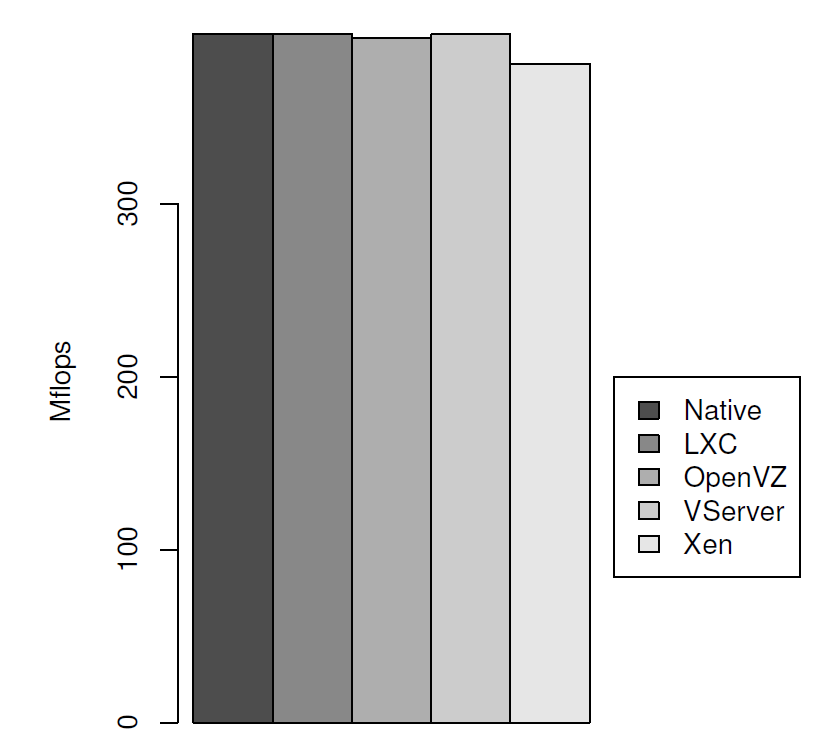
\includegraphics[width=\textwidth]{img/cpu_perf_linpack.png}
			\end{block}
		\end{column}
		\begin{column}{.5\textwidth}
			\begin{block}{\centering \textbf{Mem throughput} \\ Stream}
				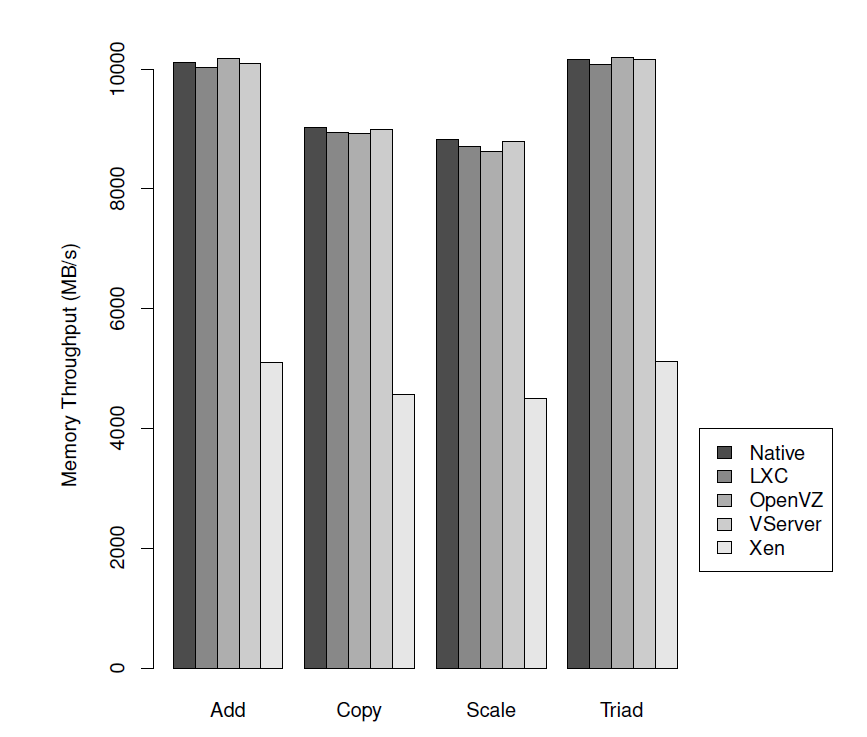
\includegraphics[width=\textwidth]{img/mem_throughput_stream.png}
			\end{block}
		\end{column}
	\end{columns}
\end{frame}

\begin{frame}{Networking Performance}
	\begin{columns}[T]
		\begin{column}{.5\textwidth}
			\begin{block}{\centering \textbf{Bandwidth} \\ NetPIPE}
				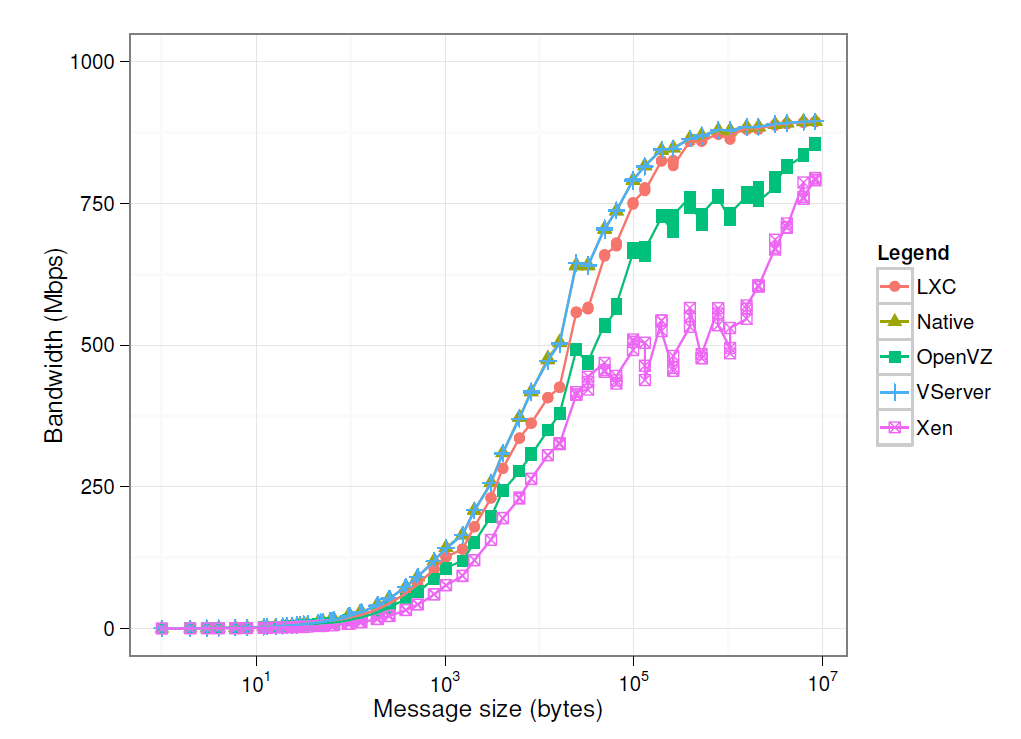
\includegraphics[width=\textwidth]{img/net_bandwidth_netpipe.png}
			\end{block}
		\end{column}
		\begin{column}{.5\textwidth}
			\begin{block}{\centering \textbf{Latency} \\ NetPIPE}
				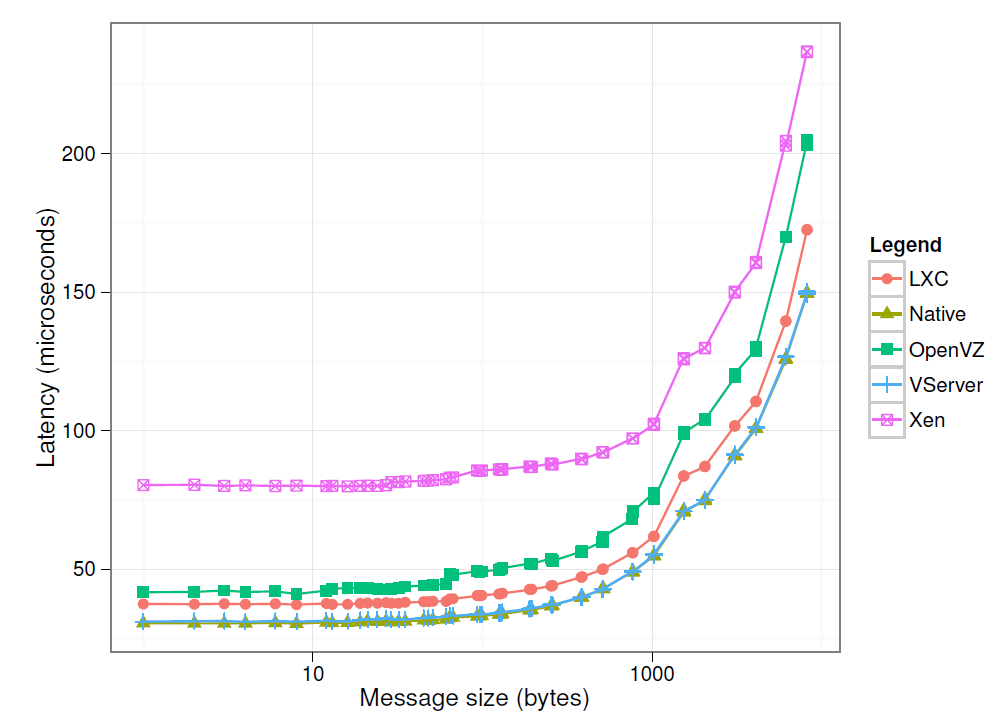
\includegraphics[width=\textwidth]{img/net_latency_netpipe.png}
			\end{block}
		\end{column}
	\end{columns}
\end{frame}

\begin{frame}{Isolation}
	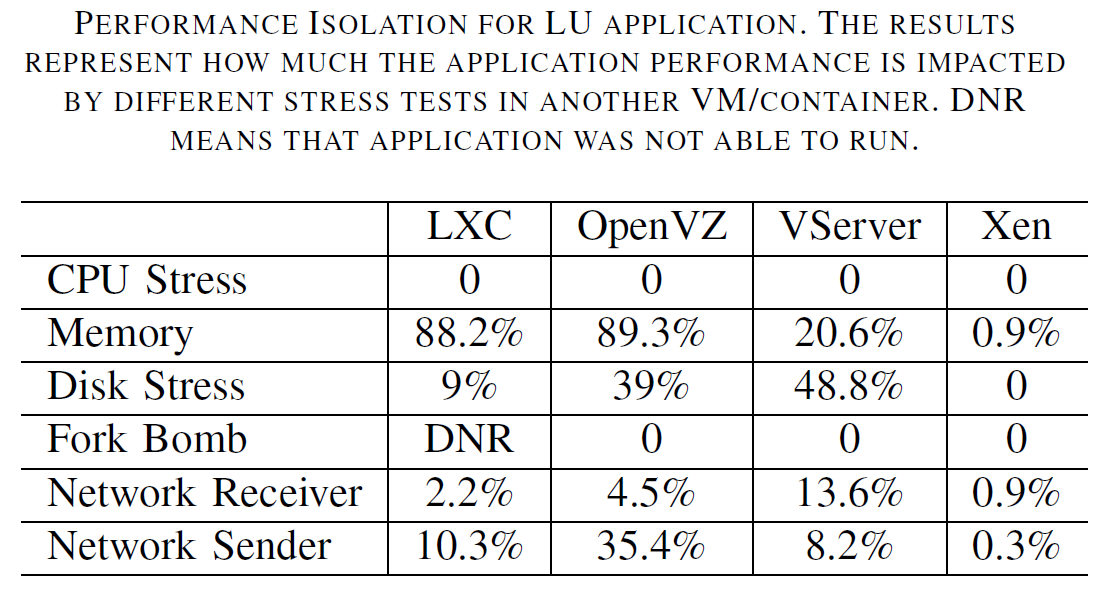
\includegraphics[width=\textwidth]{img/isolation_benchmark_suite.png}
\end{frame}

\section{Relevance}

\subsection{Spread}

\begin{frame}{Popularity}
	\begin{itemize}
	\item Running on:
		\begin{itemize}
		\item Major distros: Fedora, Debian, Ubuntu, ...
		\item Android
		\item Virtually any system with Linux >= 2.6.26
		\end{itemize}
	\item Integrated with high(er) level tools:
		\begin{itemize}
		\item \url{docker.io} - The Linux Container Runtime
		\item \url{libvirt.org} - The Virtualization API
		\item \url{criu.org} - Checkpoint-Restart in Userspace
		\end{itemize}
	\item Maintained by both kernel and userspace developers
	\end{itemize}
\end{frame}

\subsection{Use Cases}

\begin{frame}{Use Cases}
	\begin{itemize}
	\item General:
		\begin{itemize}
		\item Server replication
		\item Application sandboxing
		\item Legacy software support
		\item Live migration
		\item GPL insulation
		\end{itemize}
	\item Embedded (networking, smartphones):
		\begin{itemize}
		\item Separate traffic from different departments
		\item Separate QoS policies
		\item Run RTOS and HLOS at the same time
		\end{itemize}
	\end{itemize}
\end{frame}

\begin{frame}{Freescale USDPAA in Containers}
	\begin{itemize}
	\item DPAA - DataPath Acceleration Architecture
		\begin{itemize}
		\item HW architecture providing advanced networking capabilities
		\item Present in dedicated networking equipment
		\item Traffic shaping, package accelerators, cryptography engine
		\end{itemize}
	\item USDPAA - User Space DPAA
		\begin{itemize}
		\item Userspace drivers based on the kernel UIO framework
		\item Increased flexibility in application development
		\item Reduced risk of bugging the kernel
		\item Better error handling and system protection
		\item Performance overhead
		\end{itemize}
	\item Multiple USDPAA instances in containers
		\begin{itemize}
		\item Improved isolation
		\item Additional protection layer
		\item Finer resource tuning
		\end{itemize}
	\end{itemize}
\end{frame}

\section{QA}

\begin{frame}{References}
\begin{itemize}
\item \url{lxc.sourceforge.net}
\item Yang Yu: OS-level Virtualization and Its Applications
\item Miguel G. Xavier: Performance Evaluation of Container-based Virtualization for High Performance Computing Environments
% \item OpenVZ's: Why does the Network Namespace Suck and How to Make It Suck Faster?
% \item \url{http://www.pcgameshardware.com/screenshots/250x375/2009/05/Virtual_Windows_XP_Logo.png}
% \item \url{http://2.bp.blogspot.com/-47sakFH6uSw/UXgrhNqYF8I/AAAAAAAAHzQ/0W8zFVgR--w/s1600/lxc.png}
\end{itemize}
\end{frame}

\begin{frame}{Thank you!}
\centering
Questions?
\end{frame}

\end{document}
